\chapter{人工データ実験}
\section{シミュレーション}
ニューロン集団のカルシウムイメージングデータをシミュレーションによって作り,解析手法を評価する.
シミュレーションには1)ニューロンのネットワーク構造を作成し,2)スパイクのシミュレーションを行い,3)蛍光強度の観測データに変換する.
\subsection{ネットワーク構造}
ニューロンのネットワーク構造にはsmall world network\cite{}を用いる.
Small world networkはノード数,張り替え確率,初期次数を決めることによってネットワークを作成するアルゴリズムである.
初期次数は,ニューロンが平均何このニューロンとコネクションを持つかという変数である.
張り替え確率は,初期次数によって作成された規則的なグラフのエッジをこの確率でランダムに張り替える.
そのため,エッジのうち何割が遠くのニューロンとつながっているかを表す変数である.

ここでいうコネクティビティとは,synaptic connectivityである.
脳のコネクティビティには3種類あり,synaptic connectivityとanatomical connectivityとfunctional connectivityである.
Synaptic connetivityはニューロンがシナプスを形成してつながっている状態のことである.

実際のニューロンをsmall world networkによって表すために,初期次数と張り替え確率を実データから決める.
今回はこの値はニューロンのコネクションの割合と相互のコネクションの割合から決める.
興奮性ニューロン同士の6.7\%であり,そのうち双方向のコネクションの割合は24\%である\cite{}.
成熟したマウスの抑制性ニューロンと興奮性ニューロンのコネクションの割合は不明だが,興奮性ニューロンから抑制性ニューロンへのコネクティビティと抑制性ニューロンから興奮性ニューロンへのコネクティビティはどちらも78\%であった\cite{Holmgren2003}.
成熟したマウスではより少ないと思われるが,データが見つからなかったため,40\%とした.
相互のコネクションの割合がランダムにエッジを作るよりも高いのは,近いニューロンにコネクションが作られやすいからだと考えられる.
これらのデータを実現するように初期次数と張り替え確率を調整した.
また,抑制性ニューロン同士のコネクティビティは分からないため,興奮性と同じにしている.
\subsection{スパイクシミュレーション}
スパイクのシミュレーションにIzhikevichモデル~\cite{Izhikevich2003}を用いる.
このモデルはHodgikin-Huxleyモデルをもとにしており,計算コストが低い.
このモデルにはニューロンごとに4つのパラメータを設定する必要があり,そのパラメータでニューロンを特徴づける.
本論文では興奮性ニューロンにはregular spiking neurons,抑制性ニューロンにはfast spiking neuronsを用いる.
それらのパラメータを~\Tabref{tab:parameter1}に示す.
ただし,$r_e$と$r_i$は0から1の一様分布に従う確率変数である.

\begin{table}[htb]
  \center
  \begin{tabular}{|c|cccc|} \hline
    ニューロンの種類 & a & b & c & d \\ \hline
    興奮性ニューロン & 0.02 & 0.2 & $-65 + 15 r_e^2$ & $8 - 6r_e^2$ \\
    抑制性ニューロン & $0.02 + 0.08r_i$ & $0.25 - 0.05 r_i$ & -65 & 2 \\ \hline
  \end{tabular}
  \caption{Izhikevichモデルのパラメータ}
  \label{tab:parameter1}
\end{table}

ニューロン間でどれだけシナプス伝達が行われるかも決めなければならない.
これは隣接行列で表すことができる.
隣接行列の$(i,j)$要素は,ニューロン$j$が発火した際にどれくらいの電位がニューロン$j$からニューロン$i$に伝わるかを表す.
興奮性ニューロンからの電位は0から0.5の一様分布からサンプルし,抑制性ニューロンからの電位は-2から0の一様分布からサンプルする.

ニューロンには観測範囲外からの入力がある(以降,外部入力とする).
そのため,シミュレーション中も外部からの電位を乱数としてニューロンの電位に足す.
興奮性ニューロンは$\mathcal{N}(0,5)$に従う乱数を足し,抑制性ニューロンは$\mathcal{N}(0,2)$に従う乱数を足す.
本論文では同時に活動するニューロンを推定するのが目的の1つである.
同時に活動するニューロンは,この乱数の平均値を上げることで表現する.
外部入力の平均値を上げるとニューロンは発火しやすくなり,発火頻度が上がる.
平均値は興奮性ニューロンは1,抑制性ニューロンは0.4に上げる.

\subsection{カルシウムイメージングモデル}
スパイクデータからカルシウムイオン濃度を計算する~\cite{Vogelstein2009}のモデルを用いる:
\begin{equation}
  [Ca^{2+}]_{i,t} - [Ca^{2+}]_{i,t-1} = - \frac{\Delta}{\tau}([Ca^{2+}]_{t-1} - [Ca^{2+}]_b) + An_{i,t} + \sigma_c \sqrt{\Delta} \epsilon_{i,t},
  \label{eq:calcium}
\end{equation}
ただし,$[Ca^{2+}]_{i,t}$をニューロン$i$の時刻$t$でのカルシウムイオン濃度,$[Ca^{2+}]_b$をカルシウムイオン濃度のベースライン,$\Delta$を時間幅,$\tau$は時定数,$A$は1つのスパイクでのカルシウムイオン濃度の上がり幅,$n_{i,t} \in \{0,1\}$はニューロン$i$の時刻$t$でのスパイク,$\sigma_c$はノイズの分散,$\epsilon_{i,t} \sim \mathcal{N}(0,1)$である.
この人工データではsaturationは考えないこととする.

次に,同論文のモデルを使ってカルシウムイオン濃度$[Ca^{2+}]_{i,t}$をカルシウムイメージングで計測される蛍光強度$F_{i,t}$に変換する:
\begin{equation}
  F_{i,t} = \alpha[Ca^{2+}]_t + \beta + \sigma_F \epsilon_{i,t},
  \label{eq:intensity}
\end{equation}
$\alpha$は強度,$\beta$はバイアス,$sigma_F$はノイズの分散である.

\Tabref{tab:parameter2}に使用したパラメータを示す.

\begin{table}[htb]
  \center
  \begin{tabular}{|cccccccc|} \hline
    $[Ca^{2+}]_b$ & $\Delta$ & $\tau$ & $A$ & $\sigma_c$ & $\alpha$ & $\beta$ & $\sigma_F$ \\ \hline
    0.1 & 0.001 & 0.5 & 5.0 & 1.0 & 1.0 & 0 & 1.0 \\ \hline
  \end{tabular}
  \caption{カルシウムイメージングモデルでのパラメータ}
  \label{tab:parameter2}
\end{table}

\subsection{観測モデル}
実データは8 Hzでサンプリングされたデータなので,シミュレーションした蛍光強度を8 Hzで足し合わせる:
\begin{equation}
  x_{i,t'} = \sum_{t=1}^{125} F_{i,t}.
  \label{eq:observation}
\end{equation}

\section{結果}
\subsection{設定}
人工データは4種類作成した.
\begin{enumerate}
  \item ニューロンは1つのグループに必ず所属し,近いニューロン同士がグループとなっている
  \item ニューロンは1つのグループに必ず所属し,グループは近さに関係なくランダムに形成される
  \item ニューロンは1つか2つのグループに必ず所属し,同じニューロンが所属しているグループ同士の活動は被らない
\end{enumerate}
800個の興奮性ニューロンと200個の抑制性ニューロンについてシミュレーションを行った.
1つのグループに所属するニューロン数は50〜200個とした.
グループが活動する時間は5sごとに変えた.
シミュレーション時間は470sで,そのうちの10sは安定のため解析から除外した.

\subsection{手法の比較}
Euclidean NMF,logistic regression,glassoの性能の比較を行った.
2のタイプについて100種類のデータを生成し,ニューロン同士が同じグループにあるか否かの行列のF1 scoreを比較した.
\begin{figure}[htbp]
    \begin{center}
        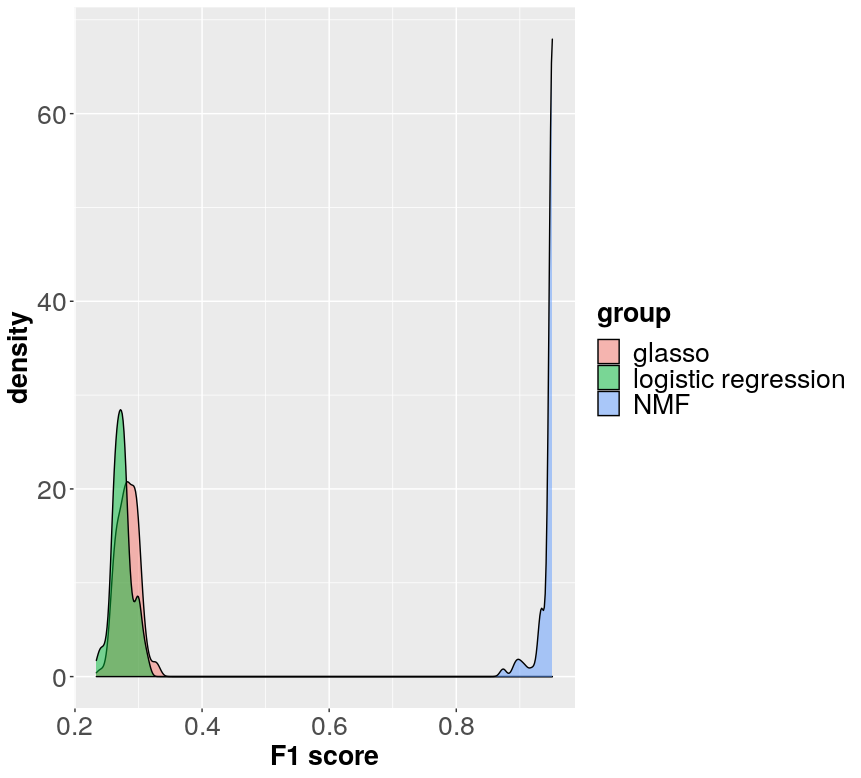
\includegraphics[width=0.5\linewidth]{compare3}
        \caption{NMF,logistic regression,glassoのF1 scoreの密度分布}
        \label{fig:compare3}
    \end{center}
\end{figure}
\Figref{fig:compare3}より,glassoとlogistic regressionの精度は低いことがわかる.
3つの手法のうちNMFがカルシウムイメージングデータを扱うのに適していると考えられる.

\subsection{推定へのネットワーク構造の影響}
グループ推定へのネットワーク構造の影響を調べるために,1と2のネットワーク構造とグループについて100種類のデータを生成し,NMFの推定精度の比較を行った.
人工データは,近いニューロンほどつながりやすい性質をもつので,1の人工データの方がニューロン同士が同期して活動しやすいと思われる.
ここで,2つのニューロンが同期するとは,一方のニューロンが発火してからごく短い間にもう一方のニューロンが発火する状態が続くことである.
実験結果を\Figref{fig:same-exc}~\ref{fig:diff-inh}に示す.
\begin{figure}[htbp]
    \begin{center}
        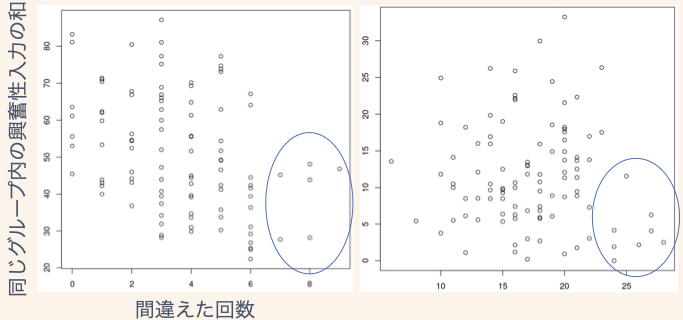
\includegraphics[width=\linewidth]{same-exc}
        \caption{データ1と2について,ニューロンごとの間違えた回数と同じグループからの興奮性入力の和の関係}
        \label{fig:same-exc}
    \end{center}
\end{figure}
\begin{figure}[htbp]
    \begin{center}
      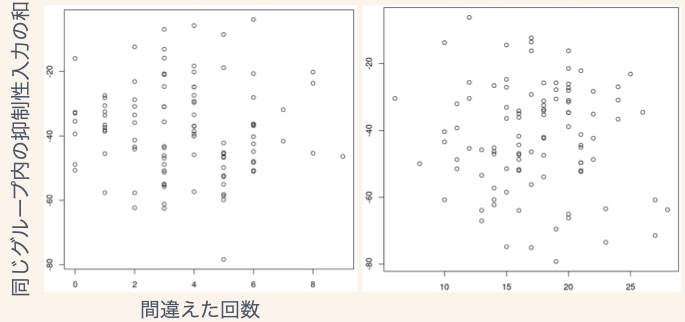
\includegraphics[width=\linewidth]{same-inh}
        \caption{データ1と2について,ニューロンごとの間違えた回数と同じグループからの抑制性入力の和の関係}
        \label{fig:same-inh}
    \end{center}
\end{figure}
\begin{figure}[htbp]
    \begin{center}
        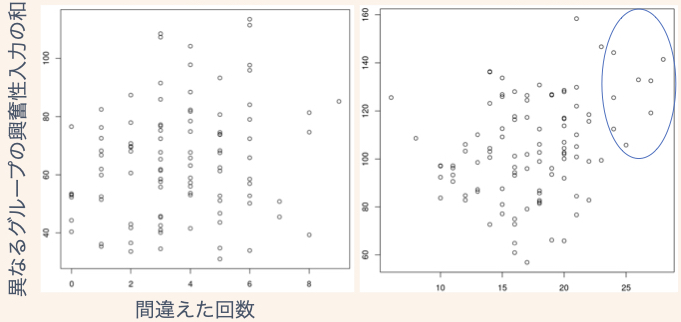
\includegraphics[width=\linewidth]{diff-exc}
        \caption{データ1と2について,ニューロンごとの間違えた回数と異なるグループからの興奮性入力の和の関係}
        \label{fig:diff-exc}
    \end{center}
\end{figure}
\begin{figure}[htbp]
    \begin{center}
        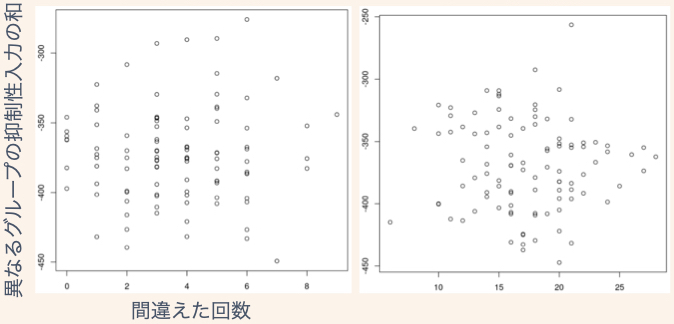
\includegraphics[width=\linewidth]{diff-inh}
        \caption{データ1と2について,ニューロンごとの間違えた回数と異なるグループからの興奮性入力の和の関係}
        \label{fig:diff-inh}
    \end{center}
\end{figure}
\Figref{fig:same-inh},\Figref{fig:diff-inh}より,抑制性の入力は間違える回数には影響しないと思われる.
\Figref{fig:same-exc}より,同じグループからの興奮性入力が小さいと間違えやすいと言える.
\Figref{fig:diff-exc}より,データ2で間違える回数が多かったニューロンは異なるグループからの興奮性入力が大きかった.
データ2ではデータ1よりも近いニューロンが異なるグループに所属する割合が多い.
そのため,異なるグループからの興奮性入力と間違える回数の関係が強く出たと思われる.

他にも推定へのネットワーク構造の影響の調査を試みたが,はっきりとした結果は得られなかった.

\subsection{ブートストラップの有用性}
1回NMFした結果とブートストラップした結果のAのF1 scoreを比較

\subsection{Model Averagingの有用性}
基底数変えてModel averageするとよかったよという話
